\documentclass[12pt,letterpaper,twocolumn,openany,nodeprecatedcode,bg=none]{dndbook}
\usepackage[english]{babel}
\usepackage[utf8]{inputenc}
\usepackage{longtable,booktabs,array}
\usepackage{calc}
\usepackage{etoolbox}
\usepackage{caption}
\AtBeginEnvironment{longtable}{\small}

% Fix for Pandoc 3.1.7+ image handling
\providecommand{\pandocbounded}[1]{#1}

% Pandoc's compact list helper
\providecommand{\tightlist}{%
  \setlength{\itemsep}{0pt}\setlength{\parskip}{0pt}}

% Remove "Figure N:" prefix from captions
\captionsetup{labelformat=empty}

% Remove section numbering
\setcounter{secnumdepth}{0}

\begin{document}

\title{Rogue}
\author{Class Handbook}
\date{}
\maketitle

\onecolumn

\emph{Your trusty class handbook for the Old Scrolls roleplaying game.}

\clearpage

\begin{figure}
\centering
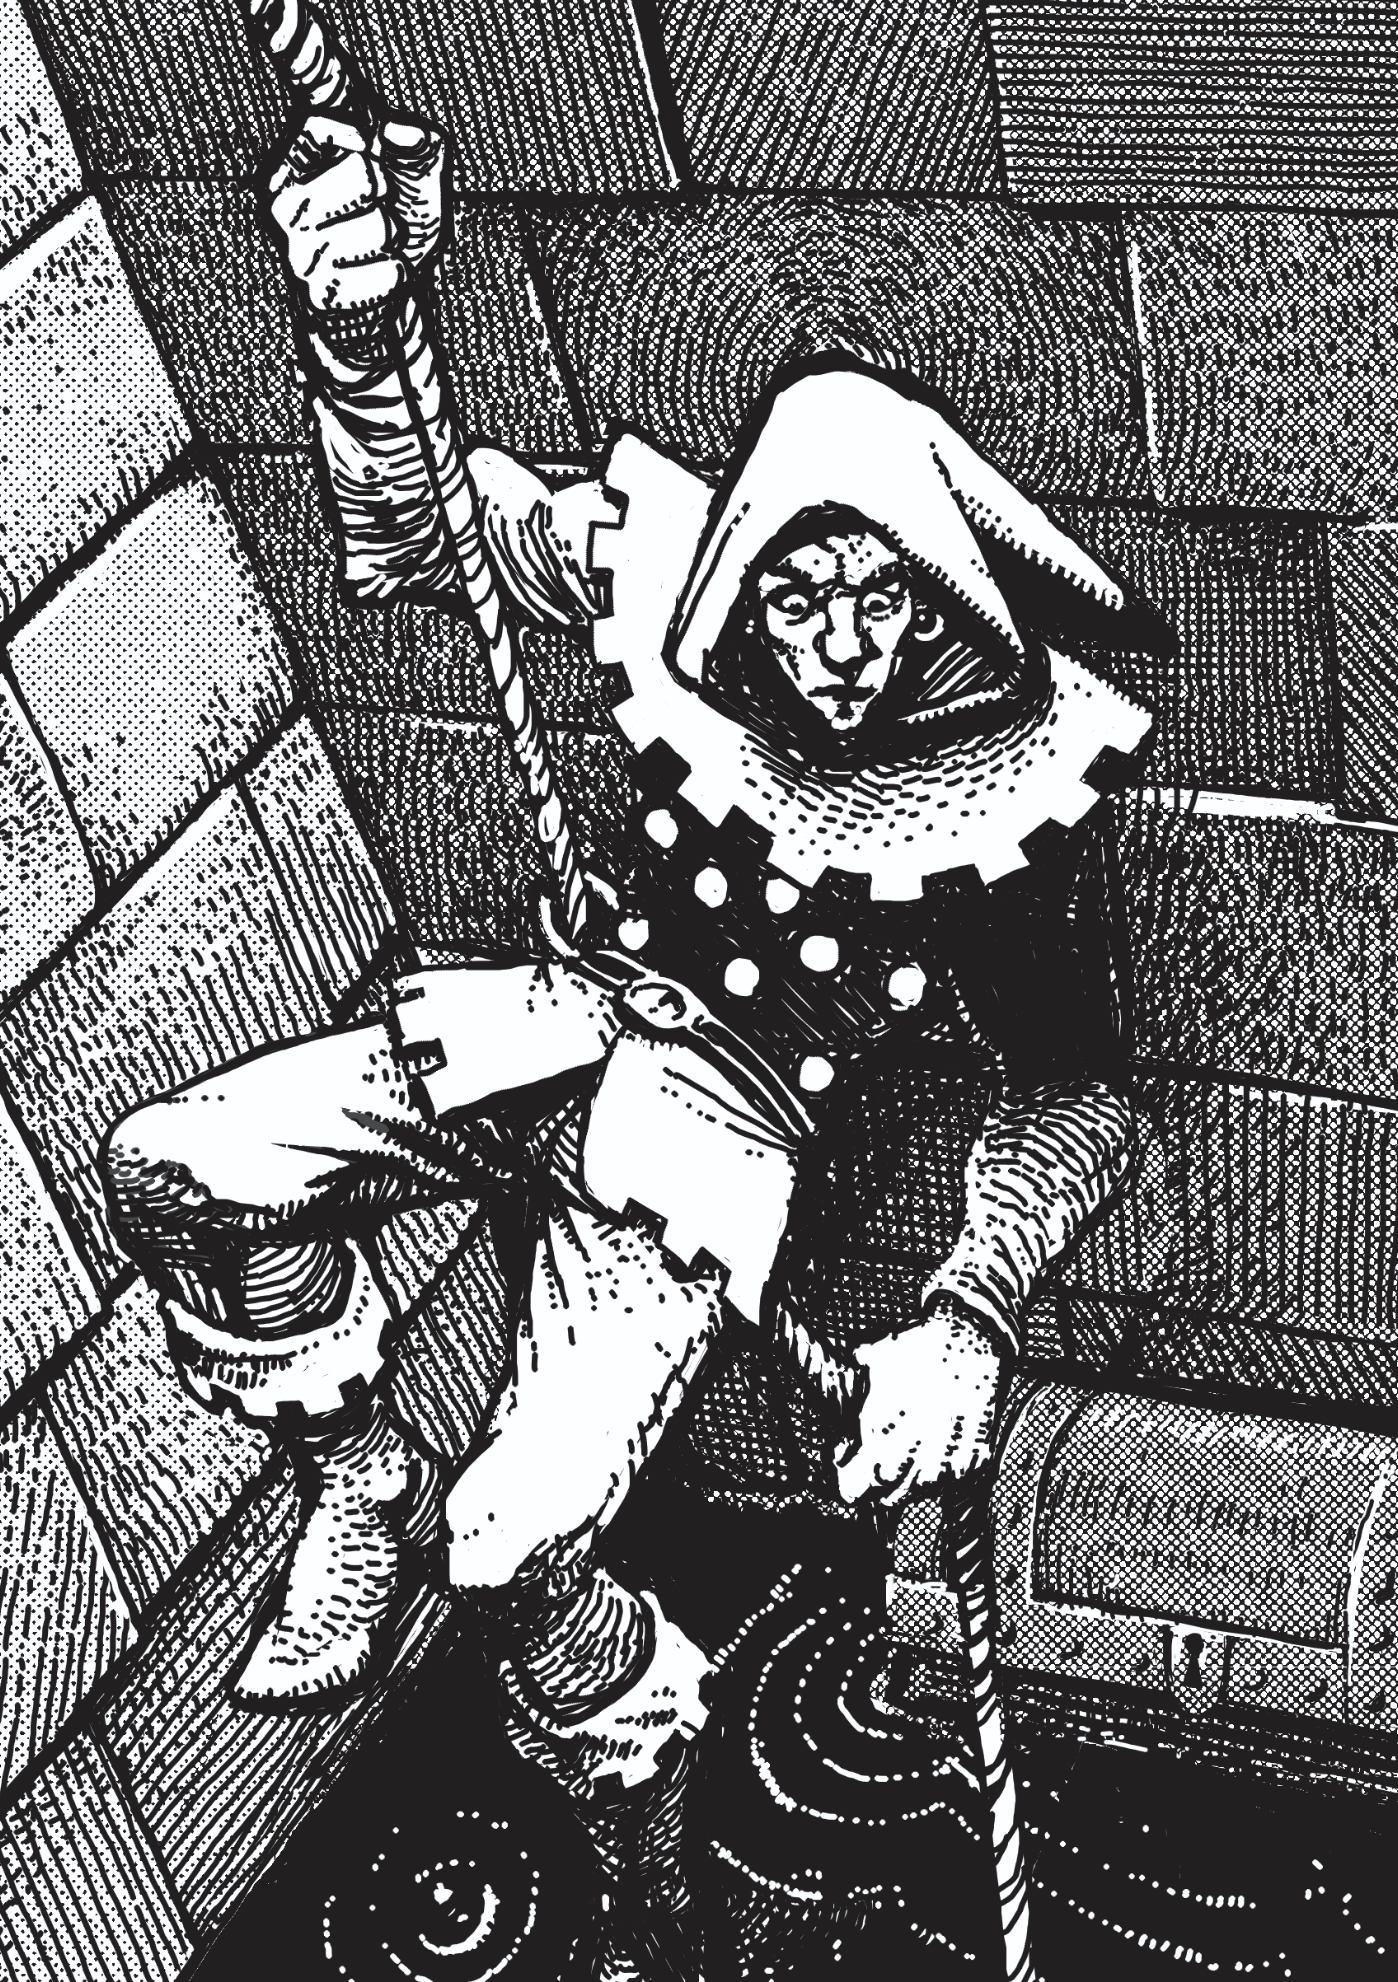
\includegraphics[width=1\linewidth,height=\textheight,keepaspectratio]{thiefSD.png}
\caption{\emph{A rogue drops into action}}
\end{figure}

\clearpage

\section{Rogue}\label{rogue}

Rogues focus on skillful strikes, movement, stealth, and mastery over
skills and knowledge rather than purely relying on raw combat ability
like the fighter does.

\subsection{Core Rogue Traits}\label{core-rogue-traits}

\begin{longtable}[]{@{}
  >{\raggedright\arraybackslash}p{(\linewidth - 2\tabcolsep) * \real{0.3333}}
  >{\raggedright\arraybackslash}p{(\linewidth - 2\tabcolsep) * \real{0.6667}}@{}}
\toprule\noalign{}
\begin{minipage}[b]{\linewidth}\raggedright
\textbf{Primary Ability}
\end{minipage} & \begin{minipage}[b]{\linewidth}\raggedright
Dexterity
\end{minipage} \\
\midrule\noalign{}
\endhead
\bottomrule\noalign{}
\endlastfoot
\textbf{Hit Points} & 10 at 1st level, 7 per level gained after 1st \\
\textbf{Saving Throw Proficiencies} & Dexterity, Intelligence \\
\textbf{Skill Proficiencies} & Choose any 4 skills \\
\textbf{Weapon Proficiencies} & Choose 3: Blade, Blunt, Bow, Mechanical,
Polearm, and Shield \\
\textbf{Starting Equipment} & Padded Jacket, 2 Daggers, Sabre, Thieves'
Tools \\
\end{longtable}

\subsection{Rogue Features Table}\label{rogue-features-table}

\begin{longtable}[]{@{}
  >{\raggedright\arraybackslash}p{(\linewidth - 6\tabcolsep) * \real{0.0568}}
  >{\raggedright\arraybackslash}p{(\linewidth - 6\tabcolsep) * \real{0.1250}}
  >{\raggedright\arraybackslash}p{(\linewidth - 6\tabcolsep) * \real{0.1364}}
  >{\raggedright\arraybackslash}p{(\linewidth - 6\tabcolsep) * \real{0.6818}}@{}}
\toprule\noalign{}
\begin{minipage}[b]{\linewidth}\raggedright
Level
\end{minipage} & \begin{minipage}[b]{\linewidth}\raggedright
Proficiency
\end{minipage} & \begin{minipage}[b]{\linewidth}\raggedright
Sneak Attack
\end{minipage} & \begin{minipage}[b]{\linewidth}\raggedright
Class Features
\end{minipage} \\
\midrule\noalign{}
\endhead
\bottomrule\noalign{}
\endlastfoot
1 & +2 & 1d6 & Roguish Archetype, Sneak Attack \\
2 & +2 & 2d6 & Cunning Action \\
3 & +2 & 3d6 & Guile (2 uses) \\
4 & +2 & 4d6 & Ability Score Improvement, Roguish Archetype \\
5 & +3 & 5d8 & Flashing Blade \\
6 & +3 & 5d8 & Ability Score Improvement, Guile (3 uses), Roguish
Archetype \\
7 & +3 & 5d10 & Expanded Skills \\
8 & +3 & 5d10 & Ability Score Improvement, Guile (4 uses) \\
9 & +4 & 5d12 & Superior Reflexes \\
10 & +4 & 5d12 & Rogue's Action \\
\end{longtable}

\twocolumn

\subsection{Rogue Features}\label{rogue-features}

As a rogue, you gain the following class features when you reach the
specified rogue levels.

\subsection{Level 1: Roguish Archetype}\label{level-1-roguish-archetype}

All rogues have a specialty, a focus for their activities that defines
their career. Pick one of the following options. Each one gives you a
special set of abilities.

\begin{itemize}
\tightlist
\item
  \textbf{Acrobat.} You gain a climb speed. You take no damage from
  falling. You can walk across surfaces as narrow as one inch, such as a
  rope.
\item
  \textbf{Arcane Trickster.} You gain a wizard cantrip of your choice
  and can cast one wizard spell. Each time you gain a level, you can
  swap those choices for different options. You use the rules for
  casting spells as per the wizard class.
\item
  \textbf{Assassin.} You are a hired killer capable of felling even the
  mightiest opponent with a single blow. You gain your Intelligence
  modifier as a bonus to damage rolls. As a search action, you can study
  a target within 30 feet. On your next turn, roll double the number of
  sneak attack dice you normally roll.
\item
  \textbf{Bard.} You know how to play two musical instruments. You gain
  a mystic cantrip of your choice and can cast one mystic spell. Each
  time you gain a level, you can swap those choices for different
  options. You use the rules for casting spells as per the mystic class.
  When you cast that spell, you cannot cast it again until you finish a
  long rest. You can use Charisma as your spellcasting ability instead
  of Wisdom.
\item
  \textbf{Brawler.} You gain an additional weapon proficiency and reduce
  the strength requirement for armor you wear by 1.
\item
  \textbf{Con Artist.} You excel at adopting various disguises and
  personas to win trust. You have advantage on all checks made to
  convince others that you are a long lost friend, comrade, or member of
  their organization.
\item
  \textbf{Pirate.} You gain an additional weapon proficiency and a swim
  speed. You know how to navigate by the constellations.
\item
  \textbf{Scout.} You gain an additional weapon proficiency and
  proficiency with the Nature and Survival skills. If you are already
  proficient with a skill gained from this feature, you gain expertise
  with it. You also know how to navigate by the constellations.
\item
  \textbf{Thief.} You gain a bonus to Stealth checks equal to your
  Intelligence modifier. If you are hidden and do anything on your turn
  to reveal yourself, you can try to hide again that turn. Normally when
  you reveal yourself you cannot try to hide again.
\end{itemize}

\subsection{Level 1: Sneak Attack}\label{level-1-sneak-attack}

Once per turn as an attack action, you can make a special attack with a
ranged or melee weapon called a sneak attack. You can also choose to use
two-weapon fighting as part of this action.

If you have advantage on the attack roll, or if at least one friendly
creature is in melee range of the target, you can deal additional damage
based on your rogue level per the Sneak Attack column on the Rogue
Features table. The extra damage's type is the same as the weapon's
type.

If neither of those conditions apply, you gain a bonus to the damage
roll equal to your level.

If the attack misses, you can apply the benefit of sneak attack to
another attack you make this turn.

\subsection{Level 2: Cunning Action}\label{level-2-cunning-action}

Your quick thinking and agility allow you to move and act quickly. On
your turn, you gain a second action called a cunning action. You can use
your cunning action to take a dash or hide action.

\subsection{Level 3: Guile}\label{level-3-guile}

In the back of your mind, you always have a plan. No matter the
situation, you have just the right tool or stratagem for the job. You
gain a pool of d20s called guile dice. You start with two dice and gain
additional dice at levels 6 and 8.

After finishing a long rest, or at the start of an adventure, you roll
each guile die. Record the results of each die. Whenever you make a
test, instead of rolling you can use one of those d20 results. When a
creature attacks you or attempts a Wisdom check to find you or discern a
lie you told, you can replace its d20 roll with one of your guile dice.

You regain all expended dice and reroll ones that you did not expend,
recording their new results, when you finish a long rest.

\textbf{Sneak Attack.} If you use guile to replace the roll of an attack
made using Sneak Attack, you damage the target as if you had advantage
on the attack, thus triggering the bonus damage.

\subsection{Level 4: Ability Score
Improvement}\label{level-4-ability-score-improvement}

You gain a +1 bonus to two abilities of your choice.

\subsection{Level 4: Roguish Archetype}\label{level-4-roguish-archetype}

You select an additional Roguish Archetype.

\subsection{Level 5: Flashing Blade}\label{level-5-flashing-blade}

When you use your sneak attack, you may make two attacks. Only one
attack gains the additional damage from sneak attack.

\subsection{Level 6: Ability Score
Improvement}\label{level-6-ability-score-improvement}

You gain a +1 bonus to two abilities of your choice.

\subsection{Level 6: Roguish Archetype}\label{level-6-roguish-archetype}

You select an additional Roguish Archetype.

\subsection{Level 7: Expanded Skills}\label{level-7-expanded-skills}

Pick two skills you do not have expertise with. If you pick a skill you
are not proficient with, you gain proficiency with it. If you pick a
skill you are proficient with, you gain expertise with it.

\subsection{Level 8: Ability Score
Improvement}\label{level-8-ability-score-improvement}

You gain a +1 bonus to two abilities of your choice.

\subsection{Level 9: Superior Reflexes}\label{level-9-superior-reflexes}

You gain expertise with Dexterity saves, allowing you to add your
proficiency bonus to Dexterity saves twice. If you already have
expertise with them, you gain expertise with a saving throw of your
choice.

\subsection{Level 10: Rogue's Action}\label{level-10-rogues-action}

Once per turn, you can expend a guile die to take an extra action that
is not a magic action or an attack action, using the die's result as the
d20 roll for any checks made as part of the action. Alternatively, when
you use Sneak Attack you can make one additional attack but must use the
die as that attack's d20 roll.

\onecolumn

\begin{figure}
\centering
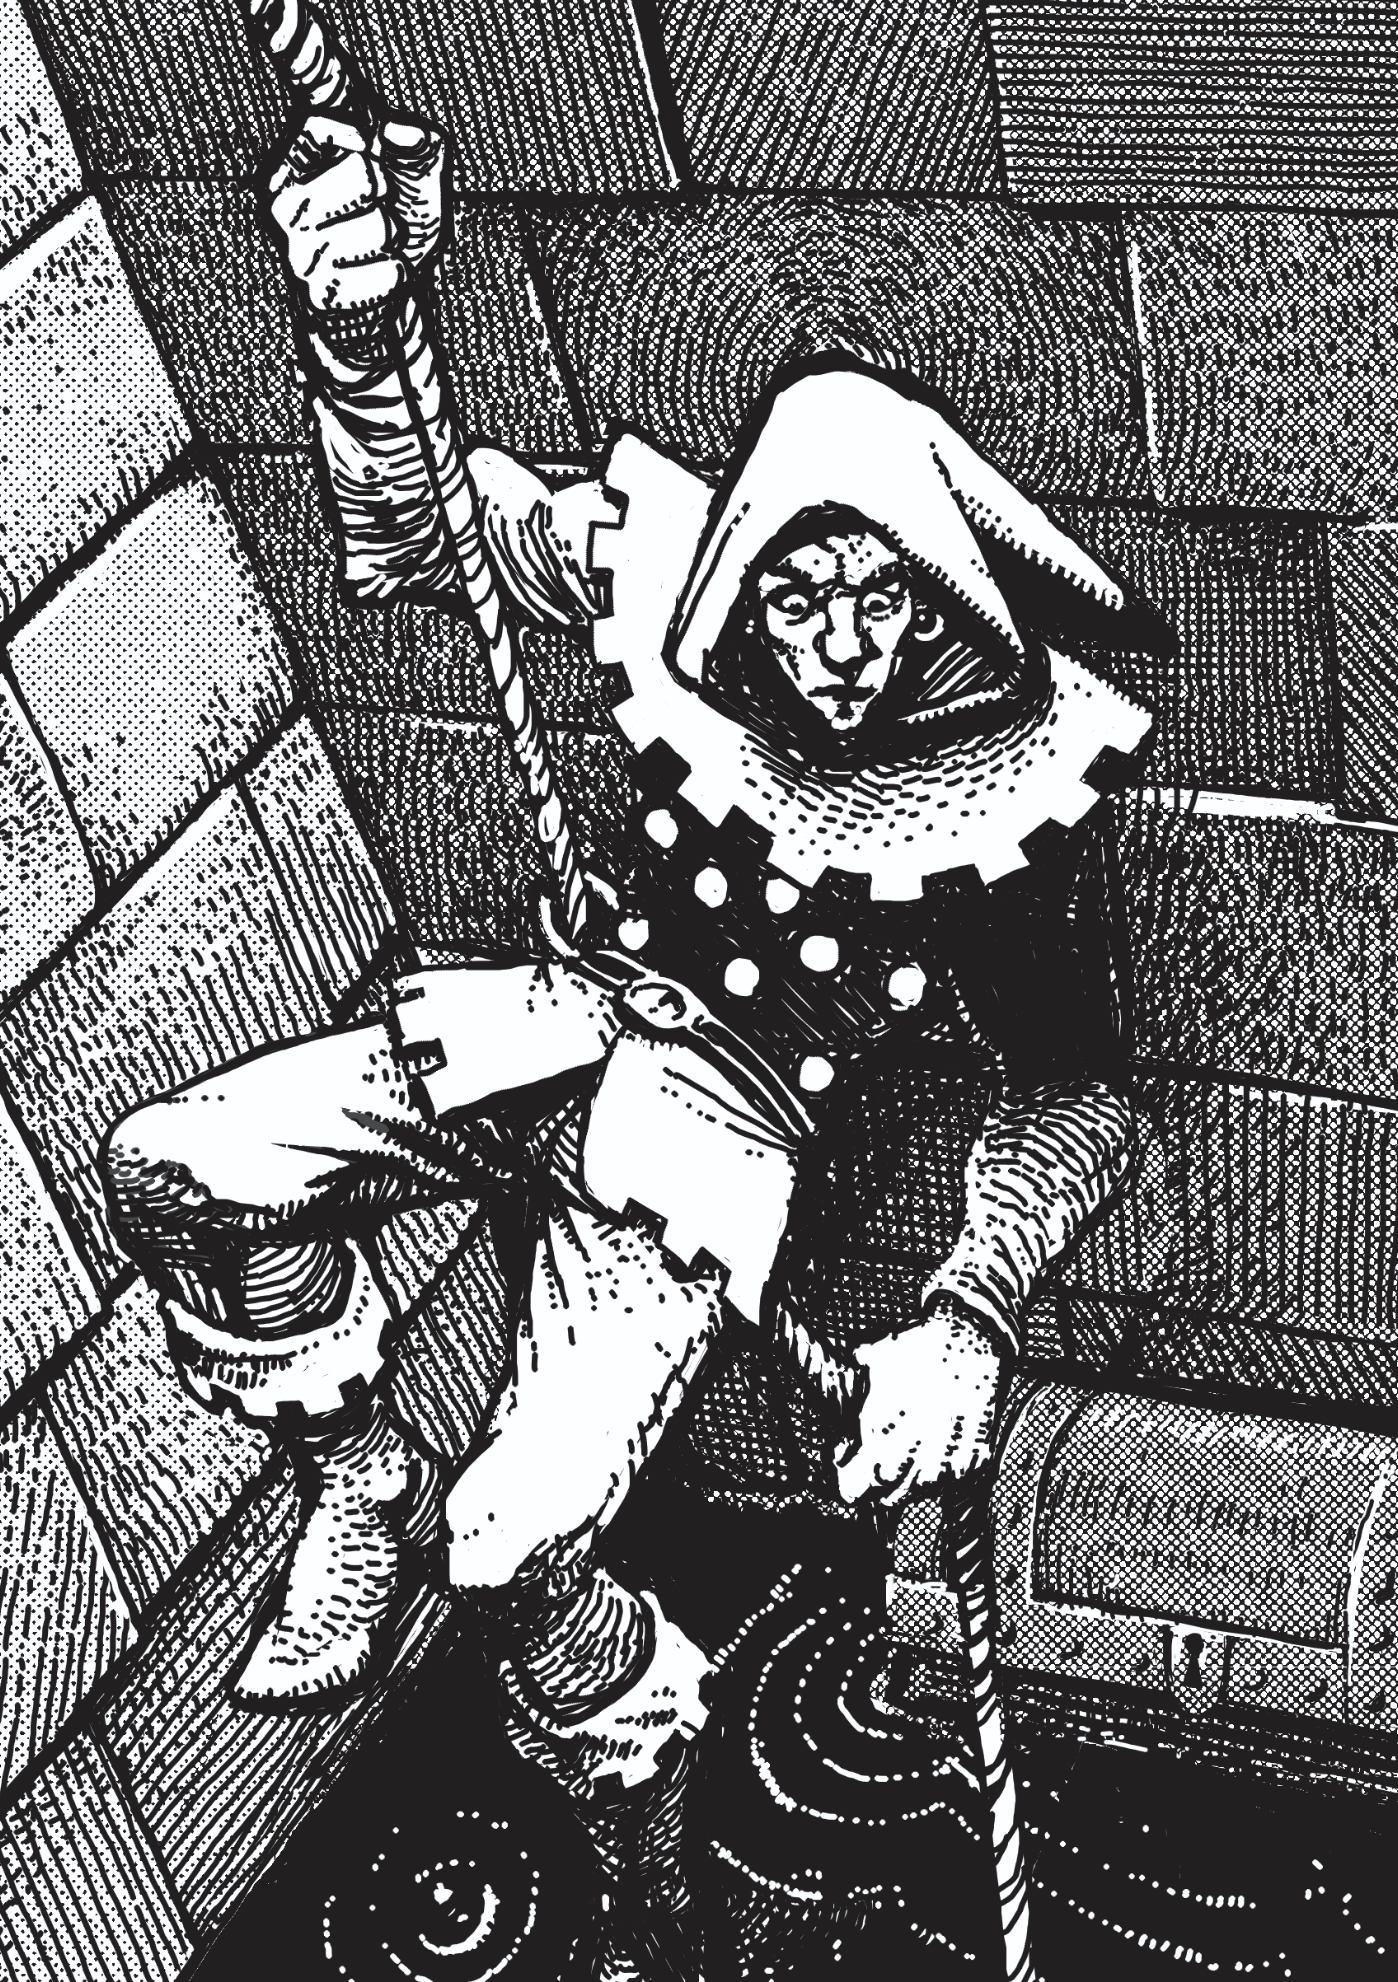
\includegraphics[width=1\linewidth,height=\textheight,keepaspectratio]{thiefSD.png}
\caption{\emph{A rogue drops into action}}
\end{figure}

\clearpage

\emph{The rogue class handbook.}

\end{document}